\section{Design Patterns}
\begin{itemize}
	\item What are Design Patterns
	\begin{itemize}
		\item Descriptions of communicating objects and classes that are customized to \textbf{\underline{solve}} a general design \textbf{\underline{problem}} in a particular \textbf{\underline{context}}
		\item 	Gamma et al. described 23 design patterns divided into three categories:
		\begin{enumerate}
			\item Creational patterns
			\item Structural patterns
			\item Behavioral patterns
		\end{enumerate}
	\end{itemize}

	\item Creational Patterns
	\begin{itemize}
		\item Concern the process of object creation
		\item Six creational patterns
		\vspace{-\itemsep}
		\begin{enumerate}
		\begin{minipage}[t]{\widthof{Abstract Factory} + 1cm}
%			\begin{enumerate}
				\item Factory Method
				\item Abstract Factory
				\item Singleton
%			\end{enumerate}
		\end{minipage}
		\begin{minipage}[t]{\widthof{Object pool} + 1cm}
%			\begin{enumerate}
				\setcounter{enumi}{3}
				\item Prototype
				\item Builder
				\item Object Pool
%			\end{enumerate}
		\end{minipage}
		\end{enumerate}
	\end{itemize}

	\item Structural Patterns
	\begin{itemize}
		\item Deal with the composition of classes or objects
		\item Seven structural patterns
		\vspace{-\itemsep}
		\begin{enumerate}
		\begin{minipage}[t]{\widthof{Composite} + 1cm}
				\item Adapter
				\item Bridge
				\item Composite
				\item Decorator
		\end{minipage}
		\begin{minipage}[t]{\widthof{Flyweight} + 1cm}
				\setcounter{enumi}{4}
				\item Facade
				\item Flyweight
				\item Proxy
		\end{minipage}
		\end{enumerate}
	\end{itemize}

	\item Behavioral Patterns
	\begin{itemize}
		\item Characterize the ways in which classes or objects interact and distribute responsibility
		\item Ten Behavioral patterns
		\begin{enumerate}
		\begin{minipage}[t]{\widthof{Chain of Responsibility} + 1cm}
				\item Chain of Responsibility
				\item Command
				\item Interpreter
				\item Iterator
				\item Mediator
		\end{minipage}
		\begin{minipage}[t]{\widthof{Observer} + 1cm}
				\setcounter{enumi}{5}
				\item Memento
				\item Observer
				\item State
				\item Strategy
				\item Template
		\end{minipage}
		\end{enumerate}
	\end{itemize}

	\item Singleton (Creational)
	\begin{itemize}
		\item Intent: Ensure a class has only one instance, and provide a global point of access to it\\
		\begin{center}
			\begin{tabular}{| l |}
				\hline
				Singleton\\
				\hline
				$ - $instance: Singleton\\
				\hline
				$ - $Singleton()\\
				+getInstance(): Singleton\\
				\ldots\\
				\hline
			\end{tabular}	\textit{	( $ - $ means private, $ + $ means public)}
		\end{center}
	\end{itemize}
	%
	\item Facade (Structural)
	\begin{itemize}
		\item Intent: Hide complexities and provide a unified interface to a set of interfaces in a subsystem\\[-10pt]
		\begin{center}
			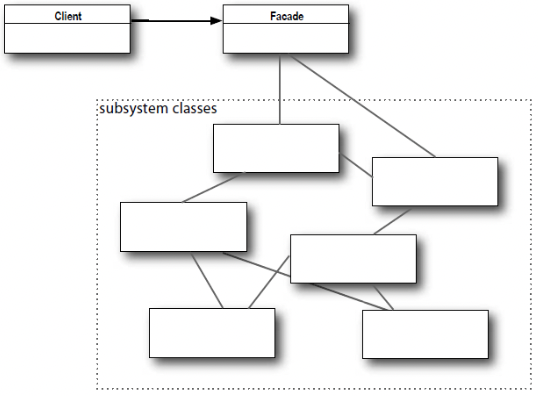
\includegraphics[scale=0.8]{Facad.png}
		\end{center}
	\end{itemize}
%	\newpage
	\item Adapter (Structural)
	\begin{itemize}
		\item Intent: Let classes work together that couldn't otherwise because of incompatible interfaces\\[-10pt]
		\begin{center}
			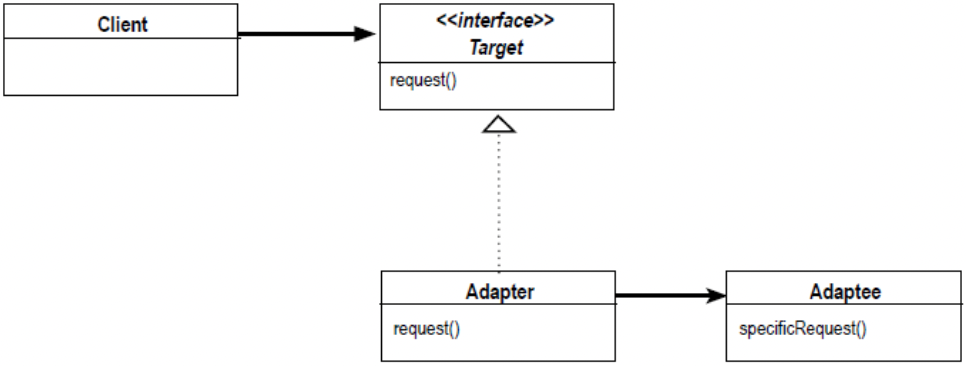
\includegraphics[scale=0.7]{Adapter.png}
		\end{center}
	\end{itemize}

	\item Observer (Behavioral)
	\begin{itemize}
		\item Intent: Define a one-to-many dependency between objects so that when one object changes state, all its dependents are notified and updated automatically\\[-10pt]
		\begin{center}
			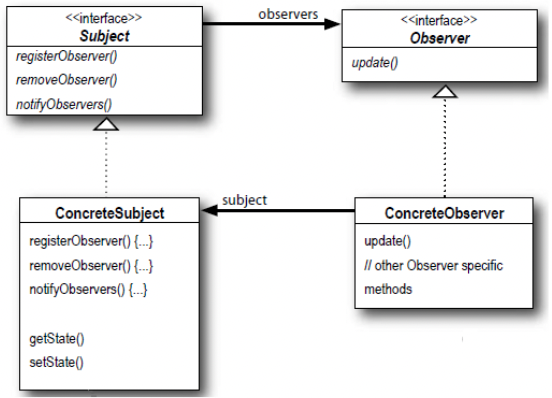
\includegraphics[scale=0.9]{Observer.png}
		\end{center}
	\end{itemize}
	%	\newpage
	\item Strategy (Behavioral)
	\begin{itemize}
		\item Intent: Define a family of algorithms, encapsulate each one, and make them interchangeable\\[-10pt]
		\begin{center}
			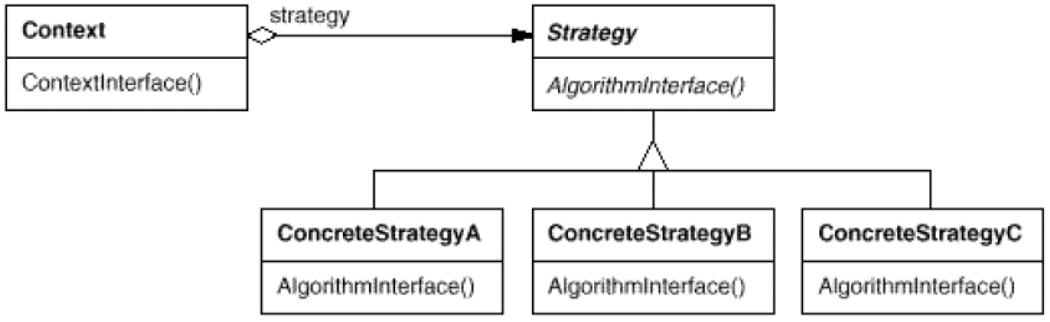
\includegraphics[scale=0.8]{Strategy.png}
		\end{center}
	\end{itemize}
\end{itemize}
